\chapter{Details and additional experiments on SHADE}
\adjustmtc
\label{chapter:shadeA}

\minitoc
\chapterwithfigures{\nameref*{chapter:shadeA}}
\chapterwithtables{\nameref*{chapter:shadeA}}

\vspace{2em}

\ifthenelse{\boolean{skipSHADE}}{\endinput}{}

In this appendix, we first provide details about the development of SHADE that were summarized in \autoref{chapter:shade}, and provide results of additional experiments conducted to validate the hypotheses made during this development.


\section{Detail on the development of SHADE}

In this section, we provide more details about the development of SHADE described in \autoref{shade:sec:model}, from the original idea of minimizing the entropy $\Ent(Y\mid \C)$ to the final loss.

\subsection{Unit-wise Entropy Regularizer}
    
\paragraph{Layer-wise regularization.} A \ac{DNN} is composed of a number $L$ of layers that transform sequentially the input. Each one can be seen as an intermediate representation variable, noted $\Y_\ell$ for layer $\ell$, that is determined by the output of the previous layer and a set of parameters $\vw_\ell$. Each layer filters out a certain part of the information from the initial input. Thus, from the data processing inequality in \citet{element} can be derived the following inequalities for any layer $\ell$:
\begin{equation}
    \Ent(\Y_\ell \mid \C) \le \Ent(\Y_{\ell-1}\mid \C) \le \cdots \le  \Ent(\Y_{1}\mid \C) \le \Ent(X\mid \C).
\end{equation}

This shows that each layer can only remove some entropy from the previous layer. What we want is to encourage the decrease in entropy. Thus, and following the recommendation of \citet{IBdeep}, we apply our regularization to all the layers, using a layer-wise criterion $\Ent(\Y_\ell \mid \C)$, and producing a global criterion to minimize:
\begin{equation}
    \Omega_{\mathrm{layers}} = \sum_{\ell = 1}^L \Ent(\Y_\ell \mid \C).
\end{equation}

\paragraph{Unit-wise regularization.} Examining one layer $\ell$, its representation variable is a random vector of $D_\ell$ coordinates $\Y_{\ell,i}$: $\Y_\ell = \left[\Y_{\ell,1}, \ldots, \Y_{\ell, D_\ell}\right]^\top$. The upper bound\footnote{This upper bound is well justified in deep learning as the neurons of a layer tend to be more and more independent of each other as we go deeper within the network.} $\Ent(\Y_\ell \mid \C) \le \sum_{i=1}^{D_\ell} \Ent(\Y_{\ell,i} \mid \C)$ enables to define a unit-wise criterion that \ac{SHADE} seeks to minimize. For each unit $i$ of every layer $\ell$ we design a loss $\omega_{\mathrm{unit}}(\Y_{\ell,i} \mid \C)=\Ent(\Y_{\ell,i} \mid \C)$ that will be part of the global regularization loss:
    \begin{align}
    \label{shadeA:SHADE}
        \Omega_{\mathrm{layers}} \le \Omega_{\mathrm{units}} = \sum_{l=1}^L \sum_{i = 1}^{D_\ell} \underbrace{\Ent(\Y_{\ell,i} \mid \C)}_{\omega_{\mathrm{unit}}(\Y_{\ell,i}\mid \C)}.
    \end{align}

Later in the chapter, we use the notation $\Y$ instead of $\Y_{\ell,i}$ for simplicity since the coordinates are all considered independently to define our criterion based on $\omega_{\mathrm{unit}}(\Y_{\ell,i}\mid \C)$. 
    
\subsection{Estimating Conditional Entropy with a Latent Code}

    In this section, we describe how to define a loss based on the measure $\Ent(\Y\mid \C)$ with $\Y$ being one coordinate variable of one layer. Defining this loss is not obvious as the gradient of $\Ent(\Y\mid \C)$ with respect to the layer's parameters may be computationally intractable. $\Y$ has an unknown distribution and without modeling it properly it is not possible to compute $\Ent(\Y\mid \C)$ precisely for the following reasons.
     
    Since $\Ent(\Y\mid \C) = \sum_{k=1}^{N_\mathrm{cls}} p(\C)\Ent(\Y\mid \C_k)$ it is necessary to compute $N_\mathrm{cls}$ different entropies $\Ent(\Y\mid \C_k)$. This means that, given a batch, the number of samples used to estimate one of these entropies is divided by $N_\mathrm{cls}$ on average which becomes particularly problematic when dealing with a large number of classes such as the 1,000 classes of ImageNet. Furthermore, entropy estimators are extremely inaccurate considering the number of samples in a batch. For example, LME estimators of entropy described by \citet{entropyestimation} converge in $\mathcal{O}(\nicefrac{(\log K)^2}{K})$ for $K$ samples. Finally, most estimators such as LME require discretizing the space in order to approximate the distribution \textit{via} a histogram. This raises issues on the bins definition considering that the variable distribution is unknown and varies during the training in addition to the fact that having a histogram for each neuron of the model is computationally and memory consuming.
    
    To tackle these drawbacks we investigate the two following workarounds: the introduction of a binary latent representation that enables to use more examples to estimate the entropy; and a bound on the entropy of the variable by an increasing function of its variance to avoid the issue of entropy estimation with a histogram and make the computation tractable and scalable.

    \paragraph{Binary latent code.}

        First, inspecting a neuron $\Y$ prior to the non-linearity, the \acs{ReLU} activation makes it act as a detector, returning a signal when a certain pattern is present on the input. If the pattern is absent the signal is zero, otherwise, it quantifies the resemblance with it.
        We therefore propose to associate a binomial variable $Z$ to each unit variable $\Y$ (before \acs{ReLU}). This variable $Z$ indicates if a particular pattern is present on the input ($Z=1$ when $\Y \gg 0$) or not ($Z=0$ when $\Y \ll 0$).
        It acts like a latent code in variational models \citep[\textit{e.g.}][]{aevb} or in generative models \citep[\textit{e.g.}][]{infogan}.
        In our implementation, we chose a binomial distribution $p(Z=1\mid \Y)=\mathrm{sigmoid}(\Y)$ that matches this intuition. 
        
        Furthermore, it is very likely that most intermediate features of a \ac{DNN} can take similar values for inputs of different classes -- this is especially true for low-level features. The semantic information provided by a feature is thus more about a particular pattern than about the class itself. Only the association of features allows determining the class. So $Z$ represents a semantically meaningful factor about the class $\C$ and from which the input $X$ is generated. The feature value $\Y$ is then a quantification of the possibility for this semantic attribute $Z$ to be present in the input or not.
        
        We assume the Markov chain $\C \rightarrow Z \rightarrow X \rightarrow \Y$. During the training, the distribution of $\Y$ varies in order to get as close as possible to a sufficient statistic of $X$ for $\C$ \citep[see definition by][]{element}. Therefore, we expect $Z$ to be such that $\Y$ draws near a sufficient statistic of $Z$ for $\C$ as well. By assuming the sufficient statistic relation $\IM(\Y, \C) = \IM(\Y, Z)$ we get the equivalent equality $\Ent(\Y\mid \C)= \Ent(\Y\mid Z)$, and finally obtain:
        \begin{equation}
            \omega_{\mathrm{unit}}(\Y\mid \C) = \Ent(\Y\mid \C)= \Ent(\Y\mid Z) = \sum_{z\in\{0,1\}} p(z) \Ent(\Y\mid Z=z).
        \end{equation}
        
        This modeling of $Z$ as a binomial variable (one for each unit) has the advantage of enabling good estimators of conditional entropy since we only divide the batch into two sets for the estimation ($z=0$ and $1$) regardless of the number of classes.
        
        
    \paragraph{Variance bound.}
        Using a binomial latent code allows computing fewer entropy estimates to obtain the global conditional entropy, thus increasing the sample size used for each entropy estimation. Unfortunately, it does not solve the bin definition issue. To address this, we propose to use the following bound on $\Ent(\Y\mid Z)$, that does not require the definition of bins:
        \begin{equation}
            \label{shadeA:variancebound}
            \Ent(\Y \mid Z) \le \frac{1}{2}\ln\big(2 \pi e \var(\Y\mid Z)\big).
        \end{equation}
        
        This bound holds for any continuous distributions $\Y$ and there is equality if the distribution is Gaussian. For many other distributions such as the exponential one, the entropy is also equal to an increasing function of the variance. In addition, one main advantage is that variance estimators are much more robust than entropy estimators, converging in $\mathcal{O}(\nicefrac{1}{K})$ for $K$ samples instead of $\mathcal{O}(\nicefrac{\log(K)^2}{K})$.
        
        Finally, the $\ln$ function being one-to-one and increasing, we only keep the simpler term $\var(\Y\mid Z)$ to design our final loss:
        \begin{equation}
            \Omega_\mathrm{SHADE} = \sum_{\ell=1}^{L}\sum_{i=1}^{D_\ell}\sum_{z \in \{0,1\}} p(Z_{\ell,i} = z \mid \Y) \var(\Y\mid Z_{\ell,i}=z).
        \end{equation}
        
        In next section, we detail the definition of the differentiable loss using $\var(\Y\mid Z)$ as a criterion computed on a mini-batch.
        
    \subsection{Instantiating SHADE}   
    \label{shadeA:instance}

        \begin{algorithm}[tb]
                \caption{\textbf{Moving average updates}:
                for $z \in \{0,1 \}$, $p^z$ estimates $p(Z = z)$ and $\mu^z$ estimates $\EE(\Y\mid Z = z)$}
                \label{shadeA:alg:maupdate}
                \begin{algorithmic}[1]
                \State \textbf{Initialize:} $\mu^0 = -1$, $\mu^1 = 1$, $p^0 = p^1 = 0.5$, $\lambda=0.8$             
                \renewcommand{\algorithmicforall}{\textbf{for each}}
                \ForAll{mini-batch $\{\yi^{(k)}, k \in 1 .. K\}$}
                    \For{$z \in \{ 0,1 \}$}
                        \State $p^{z} \leftarrow  \lambda p^{z} +   (1- \lambda)\frac{1}{K}\sum_{k=1}^K p(z\mid \yi^{(k)})$
                        \State $\mu^{z} \leftarrow \lambda  \mu^{z} +  (1-\lambda)\frac{1}{K}\sum_{k=1}^K\displaystyle \frac{p(z\mid \yi^{(k)})}{p^z}\yi^{(k)}$
                    \EndFor
                \EndFor
            \end{algorithmic}
        \end{algorithm}
        
    
        For one unit of one layer, the previous criterion writes:
        \begin{align}
        \label{shadeA:varianceDev}
            \var(\Y \mid Z) &= \int_{\mcH} p(\yi) \int_{\mcZ}p(z\mid \yi)\big(\yi-\EE(\Y\mid z)\big)^2 \dd z \dd \yi \\
            &\approx \frac 1 K \sum_{k=1}^K \left[\int_{\mcZ}p(z\mid \yi^{(k)})\big(\yi^{(k)}-\EE(\Y\mid z)\big)^2 \dd \z \right]\,;
            \label{shadeA:eq:MC}
        \end{align}
        %
        estimating the quantity $\var(\Y \mid Z)$  with Monte-Carlo sampling on a mini-batch of input-target pairs $\big\{(\vx^{(k)}, \vy^{(k)})\big\}_{1 \le k  \le K}$ of intermediate representations $\big\{\yi^{(k)}\big\}_{1 \le k \le K}$.
        
        $p(Z \mid \Y)$ interpreted as the probability of presence of attribute $Z$ on the input, it should clearly be modeled such that $p(Z = 1 \mid \Y)$ increases with $\Y$. The more similarities between the input and the pattern represented by $\Y$, the higher the probability of presence for $Z$. We suggest using:
        \begin{equation}
            \begin{cases}
                p(Z=1\mid \yi) = \sigma(\yi) \\ p(Z=0 \mid \yi) = 1- \sigma(\yi)
            \end{cases}
            \quad \text{with sigmoid function } \sigma(\yi) = \frac{1}{1 + e^{-\yi}}.
        \end{equation}
        %where $$ is the sigmoid fun\Ction. 
        
        For the expected values $\mu^z = \EE(\Y\mid z)$  we use a classic moving average that is updated after each batch as described in \autoref{shadeA:alg:maupdate}. Note that the expected values are not changed by the optimization since they have no influence on the entropy $\Ent(\Y\mid Z)$.
        
        For this proposed instantiation, our \ac{SHADE} regularization penalty takes the form:
        \begin{equation}
            \boxed{
            \Omega_{\mathrm{SHADE}} = \sum_{\ell=1}^{L}\sum_{i=1}^{D_\ell}\sum_{k=1}^K \sum_{z \in \{0,1\}} p\left(Z_{\ell,i} = z\,\middle|\, \yi_{\ell,i}^{(k)}\right) %\times \\[-3mm]
            \left({\yi_{\ell,i}^{(k)}} - \mu_{\ell,i}^ z\right)^2.
            }
        \end{equation}



\section{Additional experiments with SHADE}

Through these additional experiments, we validate the hypotheses made during the development of \ac{SHADE}, first regarding the preservation of class information by conditional entropy compare to non-conditional entropy, and second by validating of modeling of the behavior of neurons as binary detectors.

\subsection{Class-Information Preservation by Conditional Entropy}
\label{shadeA:sec:exp_cond}

\begin{figure}[tb]
    \centering
    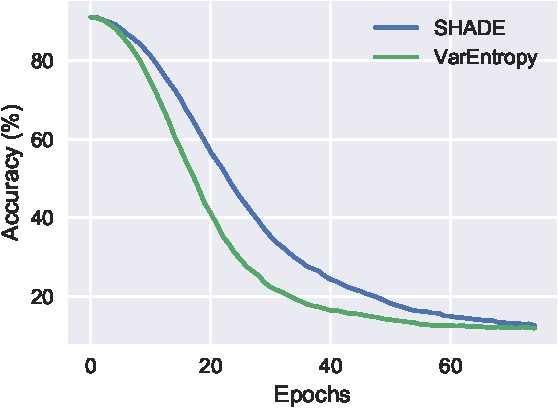
\includegraphics[width=0.55\textwidth]{images/shade_SHADE_unlearn.pdf}
    \titlecaption{Illustration of the effect of the regularization alone.}{Evolution of the accuracy of a pre-trained Inception model on CIFAR-10 when only applying regularization.}
    \label{shade:fig:unlearn}
\end{figure}

We now propose to validate our hypothesis that the introduction of our variable $Z$ is able to capture class information used for our conditional entropy.

Indeed, the main difference between \ac{SHADE} and VarEntropy is the introduction of the latent variable $Z$, supposed to contain the information about the label $\C$. The motivation of this extension is that minimizing $\Ent(\Y\mid \C)$ instead of $\Ent(\Y)$ enables to save the class information during the optimization of the regularization loss, as explained in \autoref{shade:sec:intuition}. To illustrate this benefit, we compare the impact of the two regularization losses on the classification performances of a pre-trained model. To do so, we fine tune a pre-trained Inception model only with a regularization loss, either based on $\var(\Y)$ or $\var(\Y\mid Z)$; without any label data or classification loss. The network performance obviously declines for both regularizers as we can see in \autoref{shade:fig:unlearn}. However, this decline is slower with \ac{SHADE} than VarEntropy.
This confirms the intuition that $Z$ contains class-information and that \ac{SHADE} produces less class-information filtering. This is explained by the optimization of the metric $\var(\Y\mid Z)$ that uses implicitly-learned information encoded in the network.




\subsection{Exploration of the latent representations}
\label{shadeA:sec:exp_latent}

Finally, we propose to validate our hypothesis that neurons behave as binary detectors, which motivated our binomial modeling $Z$. For this, we propose some investigations on the behavior of the activations of trained \acp{ConvNet}.

\begin{figure}[tb]
    
    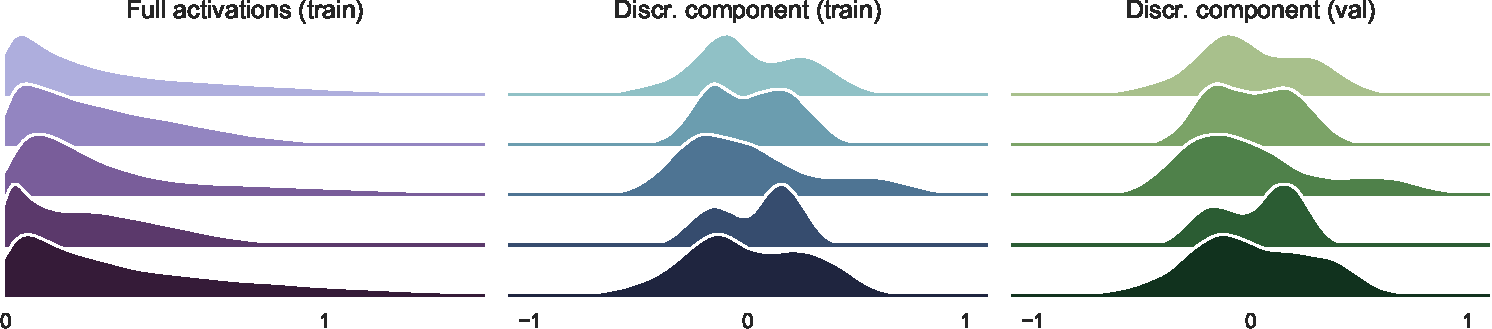
\includegraphics[width=\textwidth]{images/shade_Inception_activ}
    
    \titlecaption[c]{Visualization of 5 neurons from the penultimate activations}{(\textit{i.e.} the input of the last fully-connected layer) of an Inception model trained on CIFAR-10. On the left is the distribution of the values taken by each neuron $\Y$. In the middle and right is the distribution of the discriminiative component $\Y^*$ of the neuron (the part that does not belong to the kernel of the layer weights).}
    \label{shade:fig:activation}
\end{figure}

\paragraph{Two modes neuron variable.} First, we propose to experimentally show that \ac{DNN} optimization drives the neurons distribution toward a bi-modal distribution.

Focusing on the input neurons $\Y_{L-1}$ of the last layer of a trained network (before the class projection), the output of the network is obtained by applying a fully connected layer on $\Y_{L-1}$ plus a softmax activation: $\hat{Y} = \mathrm{Softmax}(\vW \cdot \Y_{L-1} + b)$, with $\vW$ and $b$ the weights of this layer. By plotting a histogram of any coordinate (one neuron) of $\Y_{L-1}$, it will not be possible to identify two modes. This can be seen on the purple distribution in \autoref{shade:fig:activation} (left), which represents the distributions of $\Y_{L-1,i}$ on CIFAR-10 training set for five random coordinates $i$ of an Inception model.

However $\Y_{L-1}$ contains a lot of information that will not be exploited for the prediction. Indeed, lets rewrite $\Y_{L-1} = \Y^{\bot} + \Y^*$ with $\Y^{\bot}$ in the kernel of $\vW$ such that $\vW\cdot \Y^{\bot}=0$ and $Y^*$ is in the supplementary of $\vW$'s kernel. The class space has generally much fewer dimensions than the space of $\Y_{L-1}$, thus the kernel of $\vw$ is not reduced to zero and some information will be filtered.

In \autoref{shade:fig:activation} (middle and right) is the distribution of $\Y^*$ on the training set (blue, middle) and on the validation set (green right), for the same neurons of the same network as the activations on the left. $\Y^*$ is the information effectively used for the prediction and its distribution look very much like a mixture of two Gaussians. We clearly identify two modes, one negative and one positive. This confirms the intuition of a binary latent variable $Z$ whose values correspond to the two modes. The fact that the distribution look like a mixture of two Gaussians support the use of the inequality at \autoref{shade:variancebound} in the definition of SHADE.

The distributions are obtain via a kernel density estimator using as data the neuron variable output by a forward pass on the totality of the CIFAR-10 training and test set. The three distributions are for the same coordinates taken randomly among all $\Y$ units. Note that the experiment could have been done on other layers but the computation of $\Y^*$ would be more complicated as the following transformations up to the top of the network are not linear.

\begin{table}[tb]
    \centering
    \begin{tabular}{ccccc}
    \toprule
                  & Original & \multicolumn{3}{c}{Binarized layer} \\
    \cmidrule{3-5}
    Architecture &   score   & Before $\vyh$ ($\vh_{L-1}$) & Middle ($\vh_{L/2}$) & After input ($\vh_1$) \\
    \midrule
    MLP       & 64.68 & 64.92 & 62.45 & 61.13\\
    AlexNet   & 83.25 & 82.71 & 82.38 & 82.01\\
    Inception & 91.34 & 91.41 & 90.88 & 90.21 \\
    ResNet    & 93.24 & 92.67 & 92.09 & 91.99 \\
    \bottomrule
    \end{tabular}\titlecaption[c]{Classification accuracy (\%) using binarized activation}{on CIFAR-10 test set.}
    \label{shade:table:binact}
\end{table}

\paragraph{Binary activation.}
To further demonstrate that activations in the models can be represented as a binary information, we propose to transform the \acs{ReLU} activation function of a layer into a binary activation function that can only take two values. By exhibiting that such a binary activation does not affect the accuracy, we show that we can summarize the class information of a neuron into a binary variable and still get the same prediction accuracy as with the continuous \acs{ReLU} activation. The experiment have been done on CIFAR-10 dataset with the same networks used in \autoref{shade:sec:cifar10}. 

To do this, we replace the \acs{ReLU} activation of a trained model with a binary activation function:
\begin{equation}
    \mathrm{BinAct}(H) = \begin{cases}
        0 & \text{if }H \leq 0 \\
        \overline{H^+} & \text{if }H > 0
    \end{cases}
\end{equation}
with $\overline{H^+}$ a constant value defined as the average value of the positive activations of the unit $H$.

After replacing the activation function we fine tune the layers on the top of the chosen layer, in order to adapt the top of the network to the new values and we report the obtained accuracies in \autoref{shade:table:binact} for different architecture and different layers. We note that the differences in accuracy are very small. This confirms that for a given layer, the information that is used for the class prediction can be compressed in a binary variable confirming the existence of a binary latent variable containing most of the class information that is exploited by the rest of the network. The fact that this apply for all layers of the network is consistent with the application of SHADE loss to all layers. Note that this binary activation could be further researched to improve the modeling integrated in \ac{SHADE}.
